% =====================================================================
%  Chapter 12 — Direct Detection and the Neutrino Fog
% =====================================================================

\chapter{Direct Detection and the Neutrino Fog}
\label{ch:direct}

Direct detection means looking for a dark matter particle scattering in a
target. It is the most sensitive method in the field, it is the method with
the clearest claim structure, and it has been the method with the most
complete set of null results. What follows is an account of where the
frontier is, why it has stopped where it has, and what can still be done.

\begin{figure}[!htbp]
\centering
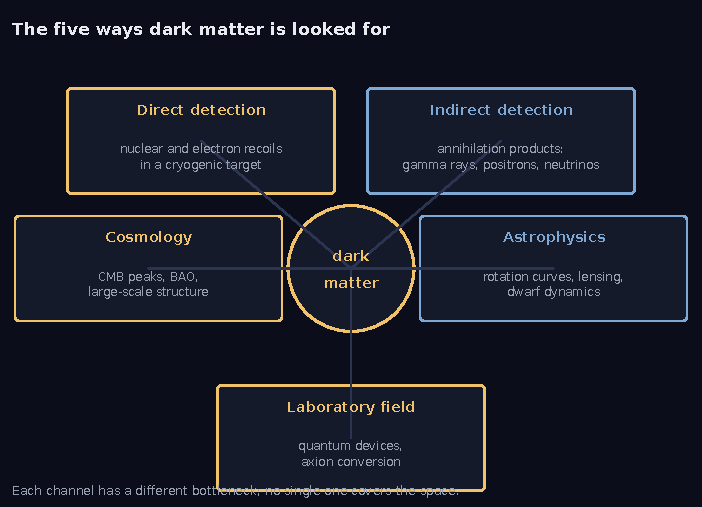
\includegraphics[width=\textwidth]{../figures/fig_channels.pdf}
\caption{The five channels through which dark matter is searched. Each
responds to a different property of the particle and carries a different
systematic floor, which is why the portfolio of Chapter~\ref{ch:portfolio}
is a requirement rather than a preference.}
\label{fig:channels}
\end{figure}

\section{The experiment}A cryogenic detector holds a kilogram-scale target --- liquid
xenon, liquid argon, or a solid --- at a temperature of a few tens of
millikelvin. A particle that scatters off a nucleus deposits a few tens of
keV of energy, which produces a burst of light in the scintillation and
a pulse of heat in the phonon system. The coincidence of the two is what
distinguishes a nuclear recoil from the radioactive backgrounds that a
detector underground still cannot fully remove.

The rate of events from a dark matter flux is a simple product: the flux,
which is set by the local density, the number of target nuclei, the
cross section, and the velocity distribution, which is what determines the
recoil spectrum. A spin-independent coupling to the nucleus gives a
coherent enhancement proportional to the square of the number of
nucleons, which is why the same flux gives a far stronger limit for heavy
targets.

\section{Where the frontier is}As of late 2026 the leading limits are:

\begin{itemize}
\item \textbf{LZ}, 4.2 tonne-year: $\sigma_{\rm SI} < 2.2\times 10^{-48}$~cm$^2$ at
40~GeV \idx{LZ Collaboration}.
\item \textbf{XENONnT}, 3.1 tonne-year: $\sigma_{\rm SI} < 1.7\times 10^{-47}$~cm$^2$ at
30~GeV \idx{XENON Collaboration}.
\item \textbf{PandaX-4T}, 1.54 tonne-year, with a comparable limit in the same
mass region \idx{PandaX Collaboration}.
\item \textbf{Light dark matter}: XENONnT's 7.8 tonne-year electron-recoil
analysis extends sensitivity to sub-GeV masses, where the recoil spectrum
is dominated by the electron cloud rather than the nucleus.
\end{itemize}

The curves are on \figref{fig:exclusions}. Two features of that figure are
the story of the last five years: the exclusion boundary has moved
downwards and to the left by roughly two orders of magnitude in cross section
over the field's lifetime, and it is now flattening at the right-hand edge
because the experiment is approaching the region where the background
dominates rather than the region where the sensitivity does.

\begin{figure}[!htbp]
\centering
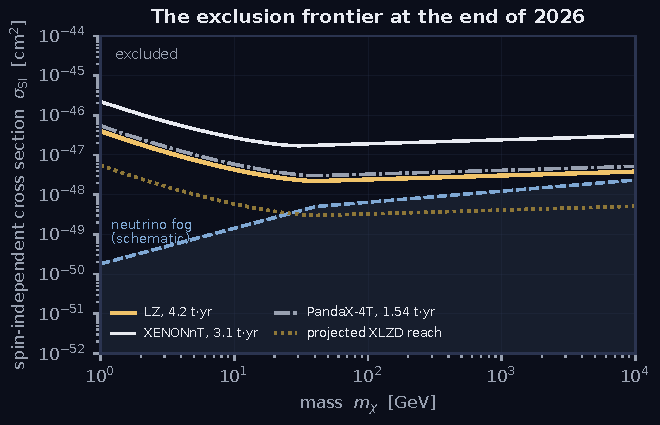
\includegraphics[width=\textwidth]{../figures/fig_exclusions.pdf}
\caption{The spin-independent nuclear-recoil exclusion frontier at the end of
2026, with the LZ, XENONnT and PandaX-4T limits and the projected reach of
the next generation. The dashed line is the neutrino fog: the flux of solar
neutrinos produces nuclear recoils indistinguishable from dark matter, and
below that line more exposure does not help.}
\label{fig:exclusions}
\end{figure}

\section{The neutrino fog}The floor in \figref{fig:exclusions} is physical, not
instrumental. The Sun's fusion chain produces neutrinos, and the
\(^{8}\mathrm{B}\) branch in particular produces neutrinos with energies of
5 to 15~MeV. Those neutrinos scatter coherently on nuclei through the
weak neutral current, producing exactly the low-energy nuclear recoils that
a WIMP search is looking for.

This is not a theoretical worry. LZ has measured the \(^{8}\mathrm{B}\) solar
neutrino CEvNS rate at 4.5~$\sigma$ \idx{LZ solar neutrinos}, and the measured
rate agrees with the Standard Solar Model. The dark matter and the neutrinos
are producing events in the same detector with the same energies and the
same spectrum.

\begin{deeper}{What the floor actually means}
The ``fog'' is a statement about the flux, not about the detector. A
detector can still push below it --- by discriminating the nuclear recoil
from the neutrino recoil using the different energy deposition of the two
processes, by going to a lighter target where the neutrino recoil spectrum
is different, or by moving to a different energy regime entirely. But in the
regime where both produce the same event in the same detector with the same
spectrum, more exposure gives no more signal, and the returns from scaling
the target mass fall off sharply. This is why the next generation is
designed around diversification rather than around tonnage.\end{deeper}

The consequence is quantitative. The 2026 Particle Data Group review puts the
practical ceiling of the xenon programme at roughly 100 tonnes of target,
with a systematic-error floor of order 1000 tonne-year, and a three-sigma
reach of about $3\times 10^{-49}\ \cmtwo$ \idx{Particle Data Group}. That is
a factor of a few better than the current best limit, not the two orders of
magnitude that the naive extrapolation from the last decade would have
suggested.

\section{What is left}Three directions remain open, and all three are
diversifications rather than extensions.

The first is \emph{light dark matter}, where the electron cloud dominates
the recoil and the interesting mass range extends down to the keV and below.
The second is \emph{electron recoil at low mass}, which the same
technologies address but with a different background and a different
systematic floor. The third is \emph{directional detection}, in which the
recoil direction carries the information that the energy alone does not,
and which the Solar System's geometry makes possible in a way it is not
possible in the deep underground.

There is also a fourth direction that is not a detection channel but a
change of instrument: the use of quantum sensors, where a single dark
matter particle produces a macroscopic quantum state change rather than a
phonon. Chapter~\ref{ch:quantum} returns to this.

\begin{keytakeaways}
\item The leading limits are LZ at $2.2\times 10^{-48}\ \cmtwo$ and
XENONnT at $1.7\times 10^{-47}\ \cmtwo$, and the exclusion boundary has
moved by two orders of magnitude in five years.
\item The floor is the solar neutrino flux, which LZ has measured at 4.5
sigma in agreement with the Standard Solar Model; it is a physical limit on
the flux, not on the detector.
\item The practical ceiling of the xenon programme is of order 100 tonnes
and $3\times 10^{-49}\ \cmtwo$, so the remaining headroom in the current
channel is a factor of a few.
\item The remaining directions --- light targets, electron recoils,
directional detection, quantum sensors --- are diversifications, and that
is the programme's real shape.
\end{keytakeaways}
